% Robin Prillwitz 2021
\documentclass[12pt,a4paper]{scrartcl}

% Robin Prillwitz 2022

\usepackage[utf8]{inputenc}
\usepackage[T1]{fontenc}

% LOCAL
\usepackage[ngerman]{babel}
\usepackage[iso,german]{isodate}
\usepackage{hyphenat}
\hyphenation{Mathe-matik wieder-gewinnen}
\usepackage[babel=true]{csquotes}

% COLOR
\usepackage[usenames,dvipsnames,svgnames,table]{xcolor}
\definecolor{hlc}{HTML}{2F4673}
\newcommand\hlc{\color{hlc}}

% FONT COLOR
% \addtokomafont{section}{\hlc}
% \addtokomafont{subsection}{\hlc}
% \addtokomafont{subsubsection}{\hlc}
% \addtokomafont{paragraph}{\hlc}
\addtokomafont{disposition}{\hlc\rmfamily}
\newcommand{\subsubsubsection}[1]{\paragraph{#1}\mbox{}\\}

% FONT
\usepackage{fontspec}
\usepackage{textcomp}
\newfontfamily\Verdana{Verdana}[Scale=MatchLowercase, Ligatures=TeX]
\newfontfamily\Helvetica{Helvetica Neue}[Scale=MatchLowercase, Ligatures=TeX]
\newfontfamily\FiraCode{Fira Code}[Scale=MatchLowercase, Ligatures=TeX]
\newfontfamily\MinionPro{Minion Pro}[Scale=MatchLowercase, Ligatures=TeX]
\setsansfont[Ligatures=TeX]{Helvetica Neue}
\setmonofont[Scale=MatchLowercase, Ligatures=TeX, Contextuals={Alternate}]{Fira Code}
\setmainfont[Ligatures=TeX]{Minion Pro}

% UTIL
\usepackage{geometry}
\usepackage[skip=12pt, indent=0pt]{parskip}
\usepackage{lipsum}
\usepackage{ragged2e}
\usepackage{seqsplit}
\usepackage{tabto}
\usepackage{setspace}
\usepackage{multicol}
\usepackage{fullpage}
\usepackage{textcomp}
\usepackage{hologo}
\usepackage{microtype}
\usepackage[inline]{enumitem}
\usepackage{url}
\usepackage{pdfpages}
%\usepackage{sectsty}

% FIGURE
\usepackage{float}
\usepackage[margin=15pt,font=footnotesize,labelfont={color=hlc,bf,sf}]{caption}
\usepackage{subcaption}
\usepackage{wrapfig}
\usepackage{bigfoot}
\interfootnotelinepenalty=10000

% GRAPHIC
\usepackage{graphicx}
\usepackage{grffile}

% TABLE
\usepackage{tabularx}
\newcolumntype{Y}{>{\centering\arraybackslash}X}
\captionsetup[table]{labelformat=simple, labelsep=colon}
\captionsetup[subtable]{labelformat=simple, labelsep=colon}

% TOC
\usepackage{tocloft}
\renewcommand{\cftsecleader}{\cftdotfill{\cftdotsep}}
\addto\captionsngerman{\renewcommand*\contentsname{Inhaltsverzeichnis}}
\addto\captionsngerman{\renewcommand*\listfigurename{Abbildungsverzeichnis}}
\setcounter{secnumdepth}{4}
\setcounter{tocdepth}{4}
% \usepackage[nottoc]{tocbibind}

% HEADER & FOOTER
\usepackage{fancyhdr}
\pagestyle{fancy}
\fancyhf{}
\renewcommand{\headrulewidth}{0pt}
\rfoot{\thepage}

% MATH
\usepackage{amsmath}
\usepackage{amssymb}
\usepackage{siunitx}

% FLOAT COUNTER
\floatstyle{ruled}
\newfloat{program}{thp}{lop}
\floatname{program}{Program}
% \newfloat{figure}{thp}{lop}
\floatname{figure}{Abbildung}
\renewcommand{\thetable}{\arabic{table}}
\renewcommand{\thefigure}{\arabic{figure}}

% TIKZ & PGF
\usepackage{tikz}
\usetikzlibrary{patterns}
\usetikzlibrary{calc}
\usetikzlibrary{shapes}
\usetikzlibrary{decorations.markings}
\usepackage{tikz-timing}
\usetikztiminglibrary[rising arrows]{clockarrows}
\usepackage{tikzpagenodes}
\usepackage[european, betterproportions]{circuitikz}
\usepackage{pgfplots}
\usepackage{pgfplotstable}
\usepackage{pgfgantt}
\pgfplotsset{
  table/search path={./data},
}
\usepackage{xparse}
\NewDocumentCommand{\busref}{som}{\texttt{%
#3%
\IfValueTF{#2}{[#2]}{}%
\IfBooleanTF{#1}{\#}{}%
}}

% APPENDIX
\usepackage[toc,page]{appendix}
\renewcommand{\appendixpagename}{Anhang}
\renewcommand{\appendixtocname}{Anhang}

% CODE
\usepackage{dirtree}
\usepackage{listings}
\renewcommand\lstlistingname{Sourcecode} % Change language of section name
\lstset{ % General setup for the package
    language=C++,
    rangeprefix=//\ ---\ ,rangesuffix=\ ---,
    includerangemarker=false,
    numberstyle=\FiraCode\color{black},
    basicstyle=\FiraCode\color{black},
    backgroundcolor=\color{White},
    keywordstyle=\color{Orchid}\bfseries,
    rulesepcolor=\color{DarkGray},
    rulecolor=\color{Black},
    stringstyle=\color{Emerald}\rmfamily,
    commentstyle=\color{LightSlateGrey},
    directivestyle={\color{RoyalPurple}},
    %
    emph={},
    emphstyle={\color{BlueViolet}},
    %
    otherkeywords = {;,<<,>>,++,|},
    keywordstyle=\color{WildStrawberry},
    numbers=left,
    frame=shadowbox,
    tabsize=4,
    columns=fixed,
    showstringspaces=true,
    showtabs=false,
    showspaces=false,
    keepspaces,
    breaklines=true,
    captionpos=b,
    title=\lstname,
    float,
    belowskip=-0.2cm
}

% LINKS
\usepackage[hidelinks]{hyperref}
\urlstyle{tt}

% Robin Prillwitz 2020

\usepackage[acronym, toc]{glossaries}
\usepackage[automake, nonumberlist, nogroupskip]{glossaries-extra}
\makeglossaries
\setabbreviationstyle[acronym]{long-short}

\newacronym{jre}{JRE}{Java Runtime Enviornment}
\newacronym{uml}{UML}{Unified Modelling Language}
\newacronym{jar}{JAR}{Java Archive}

\newglossaryentry{jfx}{name={JavaFX}, description={Java Graphikbibliothek}}
\newglossaryentry{mysql}{name={MySQL}, description={Relationale Datenbank}}
\newglossaryentry{javadoc}{name={Javadoc}, description={Java's standard Dokumentationsmethode}}
\newglossaryentry{maven}{name={Maven}, description={Build System}}

% cursive acronyms
\renewcommand*{\glstextformat}[1]{\textit{#1}}
% glossary spacing
\renewcommand\glstreepredesc{\tabto{4cm}}

\makeglossaries


\def \faculty   {Angewandte Informatik}
\def \degree    {Angewandte Informatik}
\def \title     {JAVA Programmierung FWP - 2D Plattformer}
\def \type      {Projektarbeit}
\def \class     {Javaprogrammierung AI-B6-FWP}
\def \semester  {SS2022}

\def \auditor   {Nicki Bodenschatz}

\def \authorA    {Robin Prillwitz}
\def \matrnrA    {00805291}
\def \zipA       {84326}
\def \locationA  {Falkenberg}
\def \signatureA {./img/signature.png}

\def \date      {\today}

\def \stretch {1}

\begin{document}
\setstretch{1.0}

% HEADING
\setcounter{page}{0}

% Robin Prillwitz 2020

\newgeometry{
    left=1.50cm,
    right=1.50cm,
    top=1.11cm,
    bottom=2cm
}
\begin{titlepage}
    \thispagestyle{empty}
    % draw outline
    \begin{tikz}[remember picture,overlay]
        \draw[black, line width=1pt]
        (current page text area.south west) rectangle
        (current page text area.north east);
    \end{tikz}
    % write text stuff
    \begin{center}
        {
        \Verdana
        \fontsize{14}{14.4}\selectfont
        \vspace{2.4cm}
        Technische Hochschule Deggendorf\\
        \vspace{2cm}
        Fakultät \faculty\\
        (Bachelor-Studiengang \degree)\\
        \vspace{3cm}
        \textbf{\title}\\
        \vspace{3.8cm}
        \type \\ für das Fach\\ \class\\ \semester\\
        \vspace{3.8cm}
        \fontsize{14}{24.4}\selectfont
        % lower two column stuff
        \begin{tabularx}{0.9\textwidth}{
            >{\hsize=0.9\hsize\linewidth=\hsize}X
            >{\hsize=0.5\hsize\linewidth=\hsize}X
        }
            vorgelegt von: & Erstprüfer: \\
            \authorA\;(\matrnrA), \zipA\;\locationA & \underline{\hspace*{5.5cm}} \\
            am: \date &
        \end{tabularx}
        }
    \end{center}
\end{titlepage}
\restoregeometry
\newpage


\setcounter{page}{1}
\pagenumbering{roman}
% TOC
% \addcontentsline{toc}{section}{Inhaltsverzeichnis}%
\thispagestyle{fancy}
\tableofcontents
\thispagestyle{fancy}

% % TABLES
% \addcontentsline{toc}{section}{Tabellenverzeichnis}%
% \listoftables
% \thispagestyle{fancy}

% % FIGURES
% \addcontentsline{toc}{section}{Abbildungsverzeichnis}%
% \listoffigures
% \thispagestyle{fancy}

% ACRONYMS
\setglossarystyle{listdotted}
\setglossarystyle{tree}
% \printacronyms[]
\printglossary[type=\acronymtype, title=Abkürzungsverzeichnis]
\thispagestyle{fancy}

% GLOSSARY
\printglossary
\thispagestyle{fancy}

\newpage
\setcounter{page}{1}
\pagenumbering{arabic}
\pagestyle{fancy}
\setstretch{\stretch}

% ----------------------

\section{Allgemeine Übersicht}

\textit{
Domino's Pizza® dominiert die Dystopie Düsburgs.
Kann Pizza Hut® den Ruf der runden Fressalien retten?
Begib dich zur Auslieferung an die Front und beweise deine italienischen Wurzeln!
}

Das Spiel \textit{Pizza Hut 2077} ist ein Sidescolling Jump'n'Run.
Das Spiel besteht aus einer simplen 2-Dimensionalen Welt.
Diese ist mit zufällig generierten Plattformen gefüllt.
Das konkrete Ziel des Spiels besteht lediglich in dem Highscore.
Während des Ablaufes muss der Spieler Gegnern ausweichen und sich von Platform zu Platform hangeln.
Der Spieler kann diese Gegner durch das Werfen von Pizzen eliminieren.
Die Feuerrate der Pizzen ist jedoch limitiert.
Das Spiel ist zu Ende, wenn der Spieler von einem Gegner berührt wird oder aus der Welt fällt (bzw. nicht auf einer Platform landet).
Alle dem Genre üblichen Funktionen sind wie zu erwarten realisiert.

Am Ende des Spiels kann der Spieler seinen Highscore mitsamt einem Namen in einer Datenbank speichern.
Die \gls{mysql} Datenbank ist online gehosted, darum wird eine funktionierende Internetverbindung benötigt.
In dem Credits-Bildschirm kann, mit dem notwendigen Administrator Passwort, die Highscore Tabelle der Datenbank zurückgesetzt werden.
Das einfügen von neuen Highscores zum Spielende verläuft ohne Passwort.
Die Dateneingabe hat jedoch nur Rechte zum Erstellen neuer Daten und ist auch gegen \texttt{SQL}-Injections gehärtet.

Die Hintergrundmusik des Spiels reagiert auf den jeweiligen Zustand.
Im Hauptmenü wird eine ruhigere Version des Arpeggio Leitmotivs gespielt.
Zum Spielstart geht diese mit über eine Brücke in den Hauptteil über.
Der Hauptteil wird während des Spielverlaufs gelooped.
Wenn der Spieler stirbt, wird der Hauptteil durch das Outro unterbrochen.
Der Soundtrack stammt aus eigener Komposition.
Außerdem haben die Aktionen des Spielers zugehörige Soundeffekte, wie beispielsweise beim Springen oder bei dem Werfen von Pizzen, die passend abgespielt werden.

Die Graphik des Spiels beruhen auf \gls{jfx}.
Die meisten graphischen Elemente und Animationen sind durch individuelle Sprites implementiert.
Einfache Animationen wurde durch das Abspielen verschiedener Sprites nacheinander realisiert.
Alle Sprites stammen aus eigener Produktion.
Interaktive Elemente wie Text und Eingabefelder nutzen jedoch \gls{jfx} Widgets.

Das Projekt wird mithilfe von \gls{maven} kompiliert.
Zur Ausführung ist eine funktionierende Instanz davon nicht notwendig, lediglich eine \gls{jre} von Version 18 oder später.
Da das Projekt in eine eigenständige \gls{jar} mitsamt aller Ressourcen (Sprites und Sounds) und aller notwendigen Abhängigkeiten (\gls{jfx} und Freunde) kompiliert werden kann.
Außerdem kann durch \gls{maven} eine vollwertige und interaktive Dokumentation mit \gls{javadoc} erstellt werden.
Die gesamte Codebase ist auch in der \gls{javadoc} Konvention kommentiert.

Anleitungen zur Kompilation, Steuerung und Tasten und weiteres können in der \texttt{README.md} gefunden werden.
Attribution für benutzte Ressourcen ist in der \texttt{ATTRIBUTION.md} gelistet.

\subsection{\acrshort{uml}-Diagramm}

\begin{figure}[H]
    \centering
    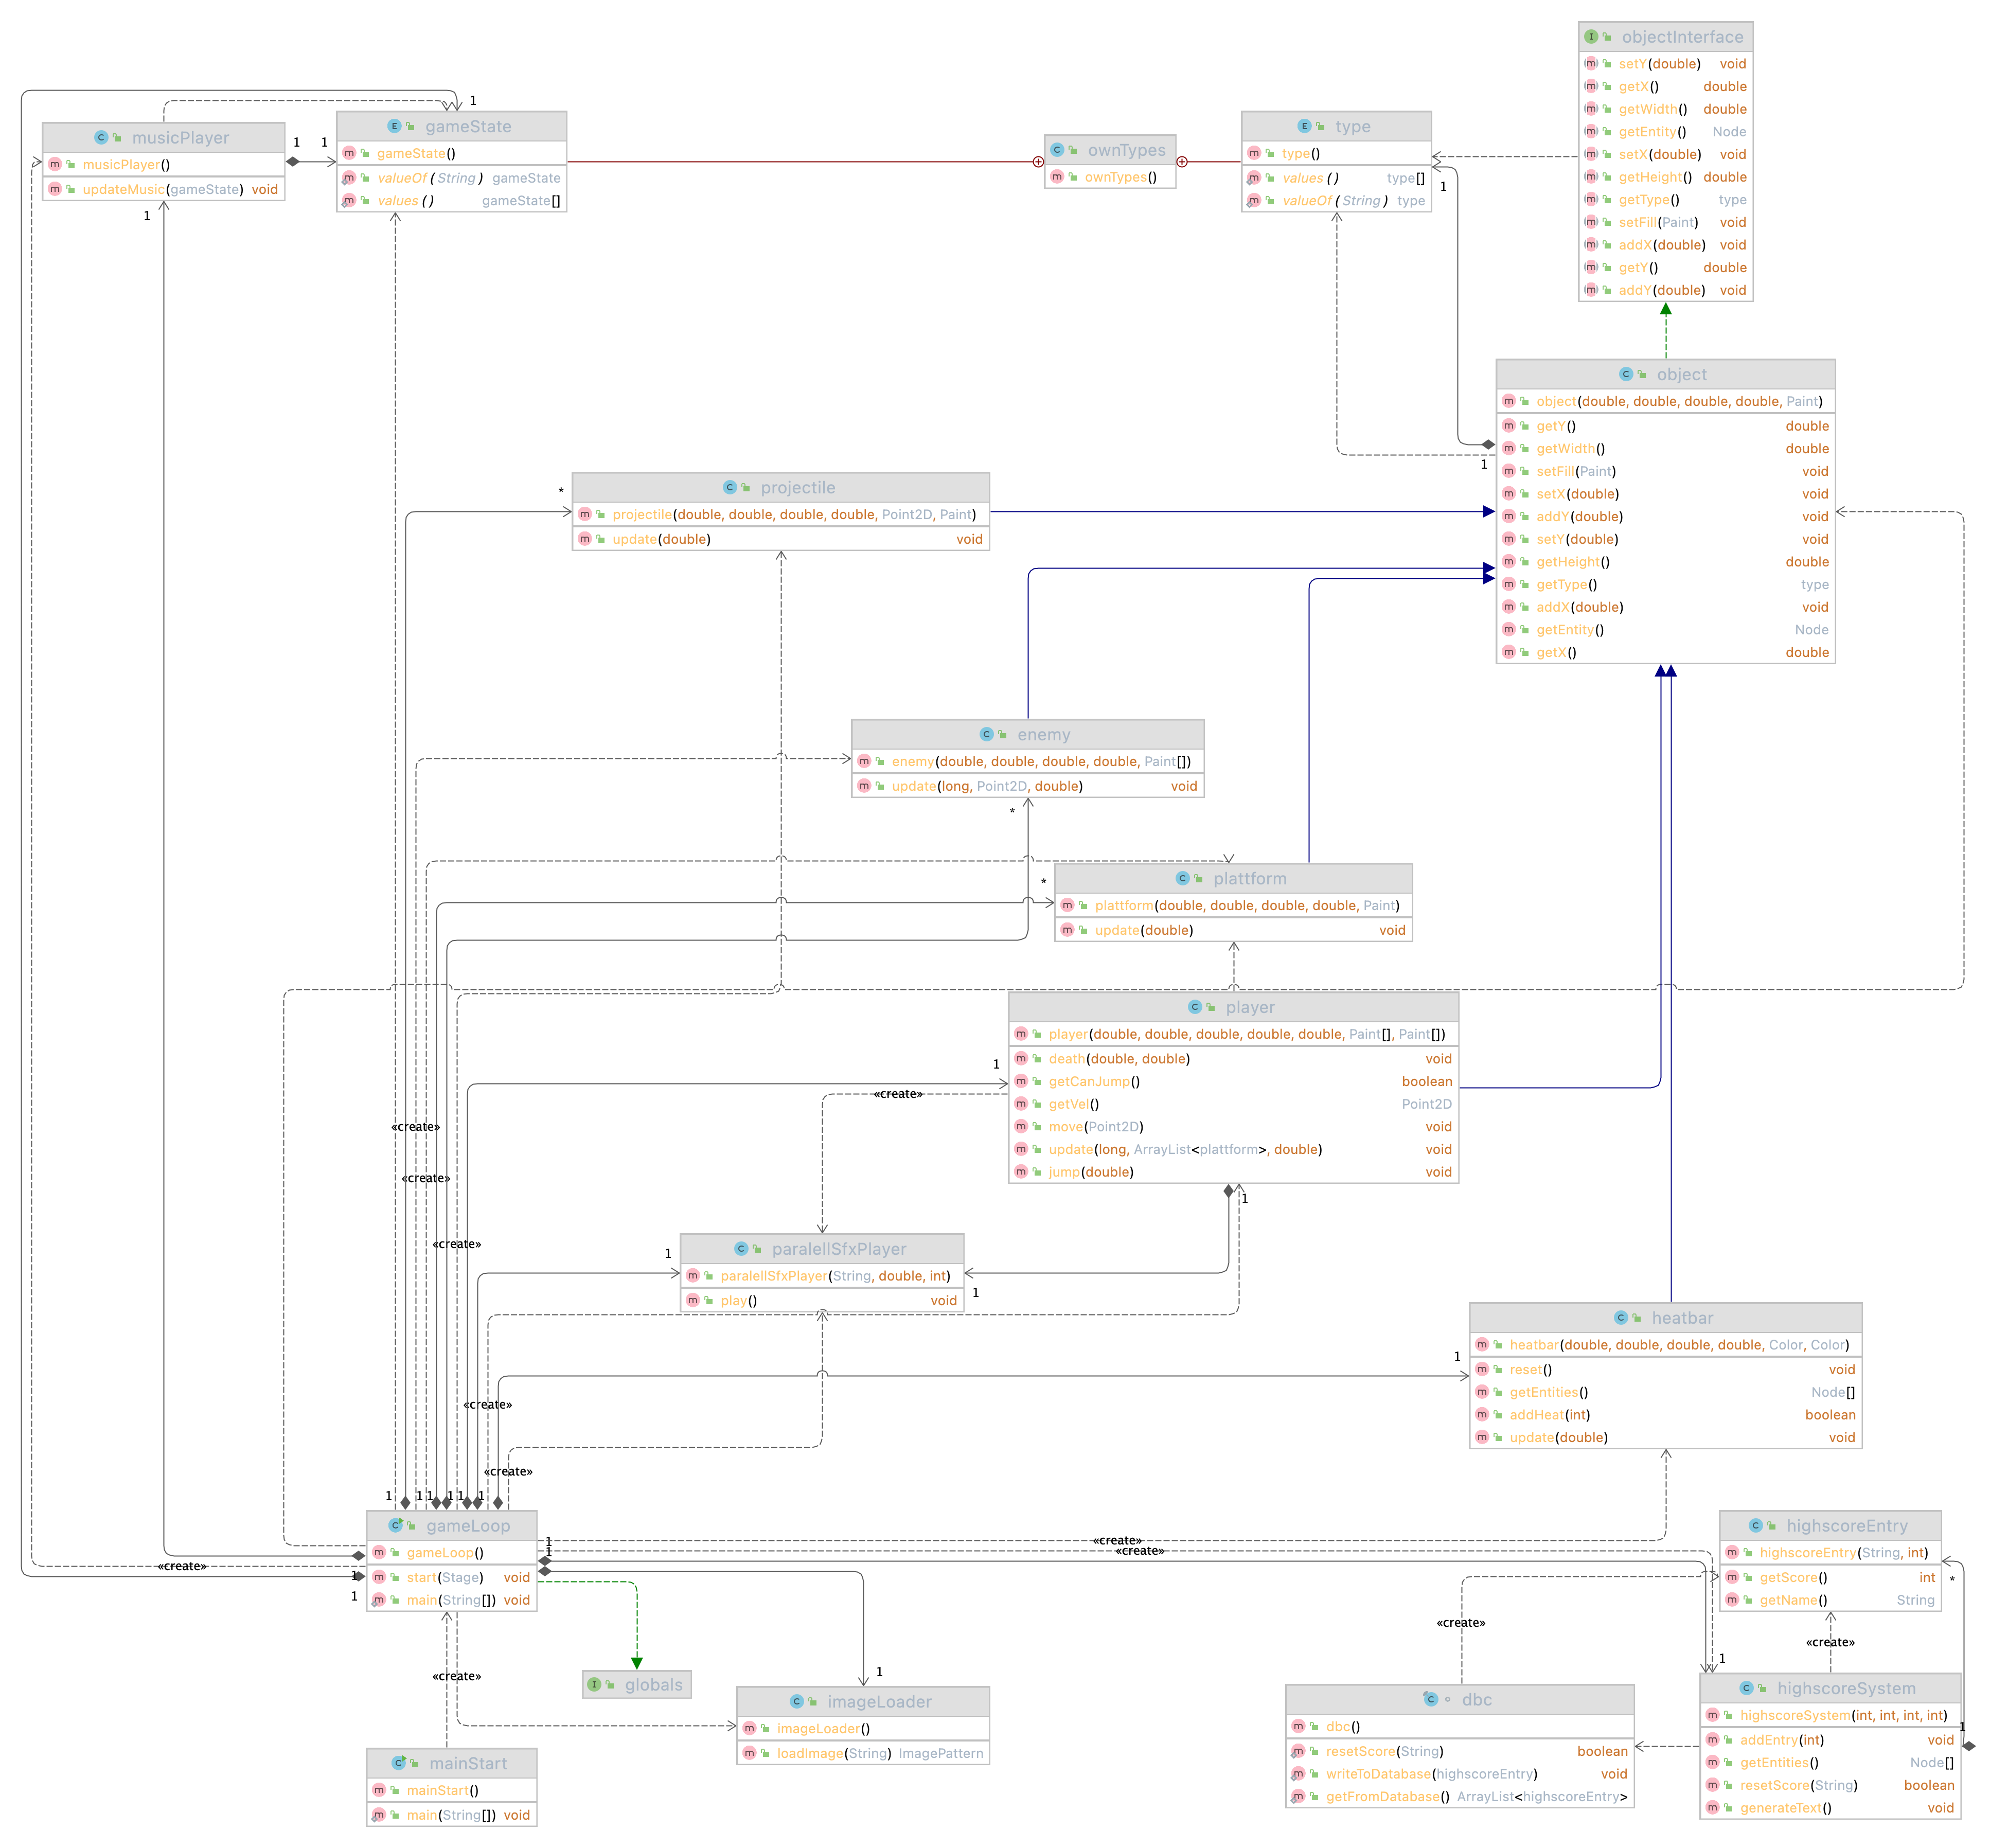
\includegraphics[width=0.9\textwidth]{img/uml.png}
    \caption{\gls{uml}-Diagramm des Projekts. Das Bild befindet sich auch im Haupt-Verzeichniss des Projekts.}
    \label{fig:uml}
\end{figure}

Das ist \autoref{fig:uml} dargestellte \gls{uml} Diagramm gibt den gesamten Inhalt des implementierten Packets an.
Äußere Abhängigkeiten werden nicht aufgeführt.
Der Großteil spielt sich in und um der Klasse \texttt{GameLoop} ab.
Die relevanten Teile der Core-Gameplay-Schleife und weiteres werden darin erstellt und aktualisiert.
Alle im Spiel auftretenden Elemente erben von der Klasse \texttt{Objekt}, welche das \texttt{ObjectInterface} implementiert.
Musik wird durch die \texttt{MusicPlayer} Klasse gehandhabt und Sound durch den \texttt{ParralellSFXPlayer}.
Bilder und Graphiken werden durch den \texttt{ImageLoader} geladen aber von den Verbrauchern selbst verwaltet.
Das Highscore System mitsamt der Datenbank Verbindung wird in \texttt{HighscoreSystem}, \texttt{HighscoreEntry} und \texttt{DBC} (DataBase Connection) implementiert.
Die Klasse \texttt{MainStart} ist eine helferklasse um die \gls{jfx} Applikation zu initialisieren.

\clearpage
\section{Eigene Beiträge}

Viele Teile des Programms, vor allem Teile der größeren Klassen, wie von \texttt{GameLoop} sind durch Kollaboration entstanden.
Kein Teil wurde ausschließlich in Isolation entwickelt.
Daher überdecken sich einige Teile möglicherweise, die genaue Einteilung wurde daher nach unserem besten Gewissen festgelegt.

\subsection{Highscore \& Datenbankverbindung}

Das Highscore System und die Datenbankverbindung ermöglichen es einen Highscore sowohl zu speichern, als auch die $n$ größten Highscores anzuzeigen.
Dabei ist $n$ in \texttt{Globals} frei einstellbar\footnote{Die Anzahl ist standardmäßig $n=10$.}.
Die Anzeige der Highscores erscheint zum Ende eines Spiels, wenn entweder weniger als $n$ Highscores existieren oder der erreichte Score größer als der kleinste ist.
Erfüllt der erreichte Score diese Kriterien, so wird der Spieler aufgefordert seinen frei wählbaren Namen anzugeben\footnote{Die Länge des Namens ist auch in \texttt{Globals} standardmäßig auf $10$ Zeichen limitiert.}.
Die Angabe des Namens ist jedoch optional, das Spiels kann auch ohne Eintragung neu gestartet werden.
Die Highscore Daten können entweder in eine Online-Datenbank oder offline in eine \gls{csv} Datei gespeichert werden.
Standardmäßig ist die Offline \gls{csv} Version eingestellt.
Das kann wieder in \texttt{Globals} verändert werden.
Die Implementation dieser gesamten Funktionalität konzentriert sich auf die Klassen \texttt{Dbc} (kurz für \textit{DataBase Connection}), \texttt{HighscoreSystem} und \texttt{HighscoreEntry}.
Außerdem hat das System Einzugsbereiche im \texttt{GameLoop}.
Zu einem wird die Anzeige daraus gestartet und erhält den aktuellen Score.
Zum anderen kann die Datenbank, egal ob online oder offline, durch eine Passworteingabe im \textit{Credits} Bildschirm zurückgesetzt bzw. gelöscht werden.
Für die Online-Datenbank wird das Administrator Passwort der Datenbank benötigt.Für die Offline-Datenbank ist es das \texttt{DefaultPassword} in \texttt{Globals}.

Die Online Datenbank ist eine \gls{mysql} Datenbank, welche mit \texttt{preparedStatements} arbeitet.
Die Offline Datenbank benutzt \textit{Apache}'s \texttt{commons-csv} Bibliothek um die Daten in eine \gls{csv} Datei zu schreiben.
Die Implementation befindet sich in \texttt{Dbc}.
Die Klasse \texttt{Dbc} ist final und hat keinen internen Zustand.
Somit werden zwar mehr Ressourcenaufrufe benötigt, jedoch wird sichergestellt, dass die angezeigten Daten stets so aktuell wie möglich sein können.

Die Klasse \texttt{HighscoreEntry} stellt einen einzelnen Highscore, ein Datenpaar aus Name und Score dar.
Diese werden im \texttt{HighscoreSystem} als Arraylist gespeichert.
Dort werden diese Daten und auch das Namenseingabefeld und die Überschrift graphisch angezeigt.
Die Texteingabe und Validierung in das Namensfeld wird auch darin gehandhabt.
Die \texttt{Dbc} wird folgend davon aufgerunfen um entweder einen neuen Highscore zu schreiben, alle geschriebenen auszulesen oder um alle zu löschen.


\subsection{Build-System}

Das Build-System des Projekts stellt das System zur Kompilation, Ausführung, Verpackung, Abhängigkeits management und der \gls{javadoc} Dokumentation dar.
Das Projekt benutzt dafür \gls{maven}.
Die Konfigurationsdatei dafür ist \texttt{pom.xml}.
Die Kommandos (auf der Kommandozeile) aus \autoref{tab:command} werden dadurch zur Verfügung gestellt.

\gls{maven} kümmert sich außerdem um die externen Abhängigkeiten, wie \gls{jfx}, \texttt{commons-csv} und \texttt{mysql-connector-java}.
Dabei werden die angegebenen Versionen bei bedarf automatisch aus dem \gls{maven} Repository heruntergeladen.

Die kompilierten Dateien und die \gls{jar} Datei sind im \texttt{./target} Unterordner anzufinden.
Es werden mehrere \glsplural{jar} erstellt.
Die relevante ist unter \texttt{\seqsplit{./target/SidescrollerGame-jar-with-dependencies.jar}}.
Aufgrund der \gls{jfx} Abhängigkeiten ist diese leider nicht Platformagnostisch.
Ergo kann diese nur auf dem Betriebssystem / der Prozessorarchitektur auf der sie erstellt wurde ausgeführt werden \footnote{Dies wurde getestet zwischen einem x86 Windows 10 Computer und einem Apple M1 MacBook Pro.}.
Die \gls{jar} kann jedoch ohne \gls{jdk}, nur mit \gls{jre}, ausgeführt werden, da alle Abhängigkeiten und Ressourcen inkludiert werden.
Das hebt jedoch die Dateigröße auf rund $27$ Megabyte an.

Die \glsplural{javadoc} ist in \texttt{./javadoc} anzufinden.
Diese beziehen sich dabei auf die \gls{javadoc} Kommentare im Code.
Außerdem wird zu jeder Klasse in der interaktiven \gls{html} Dokumentation ein kleines \gls{uml}-Diagramm generiert.
Die passiert durch das \texttt{umldoclet} Plugin von \texttt{talsmasoftware}.
Die Dokumentation kann mit \texttt{./javadoc/index.html} durch jeden Browser geöffnet werden.

\begin{table}[h]
\centering
\begin{tabularx}{0.8\textwidth}{|l|X|}
    \hline
    \textbf{Kommando} & \textbf{Bedeutung} \\
    \hline
    \texttt{mvn clean} & Löscht alle Build-Artefakte \\
    \texttt{mvn compile} & Kompiliert das Projekt \\
    \texttt{mvn package} & Kompiliert und Erstellt eine \gls{jar} Datei \\
    \texttt{mvn exec:java} & Kompiliert und führt das Projekt aus \\
    \texttt{mvn javadoc:javadoc} & Erstellt die interaktive \acrshort{html} Dokumentation \\
    \hline
\end{tabularx}
\caption{\gls{maven} Kommandos}
\label{tab:command}
\end{table}


\subsection{Graphik \& Animationen}

Alle Bilder und Animationen werden durch Sprites implementiert.
Diese sind im \texttt{sprites} Unterordner anzutreffen.
Sie wurden durch \textit{Adobe Photoshop}, \textit{After Effects} und \textit{Media Encoder} erstellt.
Bilder könenn durch den \texttt{ImageLoader} geladen werden.
Diese greift auf Dateien zu, daher stand die Implementation sehr in Verbindung mit dem Build-System.
Es musste sichergestellt werden, dass die zu ladenenden Bilder auch in der \gls{jar} zugänglich sind.

Der \texttt{ImageLoader} läd Sprites so, dass diese durch die implizite Skalierung bei der Anwendung der Sprites auf ein Graphikobjekt ohne Anti-Aliasing skaliert werden.
Dadurch ersteht der Effekt, dass alle Sprites, egal wie groß, eine annehmbare Größe annehmen und dabei auch piexeliert werden.
Das hilft sofern, dass eigene Piexl-Art tatsächlich auf den Dimensionen der Piexl gezeichnet werden kann und zum Export nicht skaliert werden muss.
Beispielsweise können die Spieler Sprites im Format von $16 \times 16$ Pixel gezeichnet und gespiechert werden, die Hintergründe können aber wesentlich größer sein.
Im Spiel nehmen beide jedoch eine vergleichbare Sklaierung an.

Animationen zwischen mehrern Sprites können im Spieler, den Projektielen, den Gegener und im Hauptmenü gefunden werden.
Die Animationen bestehen aus einem einfachen Timer, welcher nach definierter Zeit die Sprite wechselt.
Der Spieler verfügt über zwei verschiedene Animationszustände: Ein \textit{Idle} und ein \textit{Running} Zustand.
Je nach der momentanen geschwindigkeit des Spielers werden die stationäre \textit{Idle} Animation oder die bewegende \textit{Running} Animation benutzt.


\subsection{Musik \& Sounddesign}

Die Musik wurde in \textit{Ableton Live} komponiert und in \textit{Adobe Audition} gemischt und gemastert.
Die Musik wurde für das Spiel in vier Teilen arrangiert:
Zuerst ein wiederholbarer Intro-Abschnitt, gefolgt von eienr Brücke, die den Übergang zum wiederholbarern Hauptteil bildet und schließlich einen Schlussteil, welcher den Hauptteil zu jedem Zeitpunkt unterbrechen kann.
Die einzelnen Sektionen wurden dannach einzelnen exportiert.

Die Soundeffekte wurden auch in \textit{Ableton Live} erstellt.
Es gibt Effekte für springen, projektiele werfen, gegener zerstören und punkte erlangen.
Die Lautstärke jedes Soundeffekts wurde im Code so angepasst, dass diese sich in die Klanglandschaft integrieren und nicht dominieren.
Alle Sounds und Musik ist im \texttt{./sound} Ordner gespeichert.



% ----------------------

\clearpage
\newpage

\begin{samepage}
% EIDENSTAT
% Robin Prillwitz 2020

\newpage
\begin{samepage}
\section*{Eidesstattliche Versicherung}
\addcontentsline{toc}{section}{Eidesstattliche Versicherung}
\vspace{0.5cm}
Ich, \underline{\textbf{\;\authorA, \matrnrA\;}}\\
\hspace*{0.8cm}\small(Vorname, Name, Matr.-Nr.)\normalsize\\[1em]
versichere an Eides Statt durch meine Unterschrift, dass ich die vorstehende Arbeit selbständig und ohne fremde Hilfe angefertigt und alle Stellen, die ich wörtlich oder dem Sinne nach aus Veröffentlichungen entnommen habe, als solche kenntlich gemacht habe, mich auch keiner anderen als der angegebenen Literatur oder sonstiger Hilfsmittel bedient habe.

Ich versichere an Eides Statt, dass ich die vorgenannten Angaben nach bestem Wissen und Gewissen gemacht habe und dass die Angaben der Wahrheit entsprechen und ich nichts verschwiegen habe.

Die Strafbarkeit einer falschen eidesstattlichen Versicherung ist mir bekannt, namentlich die Strafandrohung gemä\ss~\S~156 StGB bis zu drei Jahren Freiheitsstrafe oder Geldstrafe bei vorsätzlicher Begehung der Tat bzw. gemä\ss~\S~163 Abs.1 StGB bis zu einem Jahr Freiheitsstrafe oder Geldstrafe bei fahrlässiger Begehung.

% \vspace{-0.5cm}
\begin{table}[ht!]
    \centering
    \begin{tabular*}{\textwidth}{l @{\extracolsep{\fill}} l}
        \underline{\textbf{\;\zipA\;\locationA, \date\;}}&
        \underline{
            \includegraphics[width=5cm, trim={0 2cm 0 0}]{\signatureA}
        }\\
        Ort, Datum & Unterschrift
    \end{tabular*}
\end{table}
\end{samepage}


% COLOPHON
\vspace*{\fill}
{
\section*{\normalsize Kolophon}
\vspace*{-10pt}\noindent
{\parskip=0pt
\makebox[\linewidth][s]{Dieses Dokument ist ein \hologo{LaTeX2e}~(\fmtversion) Dokument der \hologo{KOMAScript} Klasse.}\par\noindent
\makebox[\linewidth][s]{Alle eigenen Zeichnungen sind mit Ti\textit{k}Z gesetzt. Kompiliert wurde es mit \hologo{XeLaTeX}}\par\noindent
\makebox[\linewidth][s]{und \hologo{biber} \textit{2.17} mithilfe von \hologo{TeX}~Live auf {\Helvetica macOs 12.4} am \today.}
}
}

\end{samepage}

\end{document}
